\begin{figure}[ht]
\centering
\vspace{-6mm}
\centerline{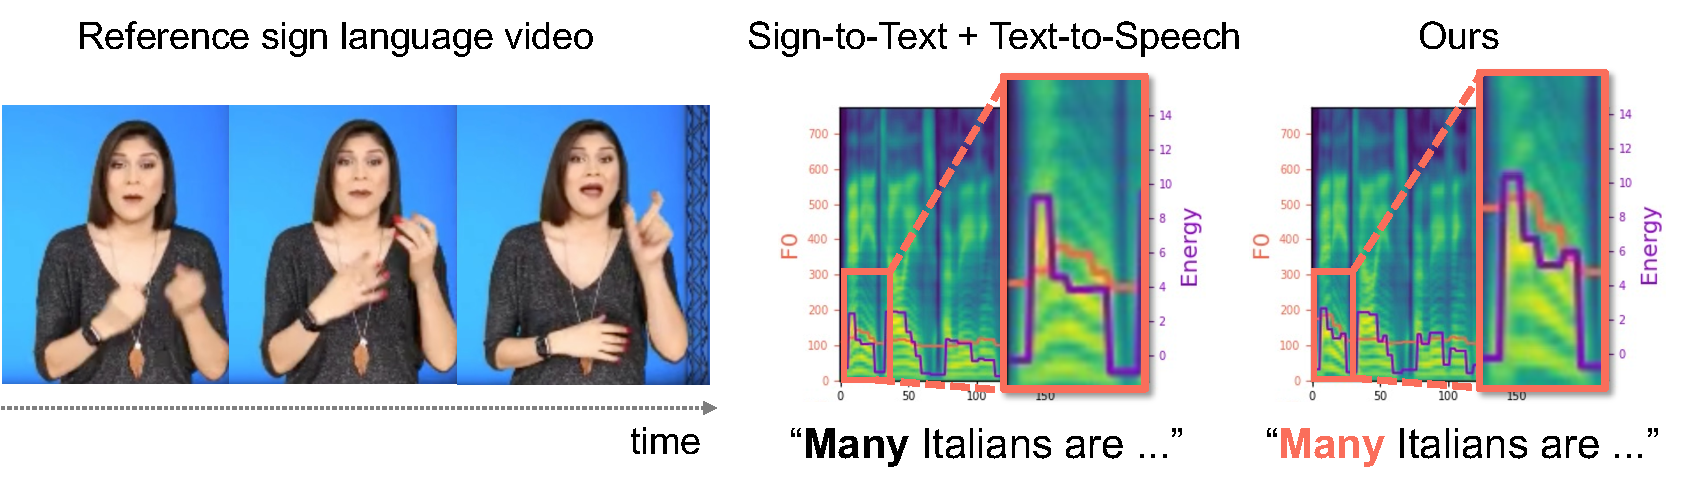
\includegraphics[width=\linewidth]{assets/heading.pdf}}
\vspace{-5mm}
\caption{
% We propose S2PFormer for \emph{Sign-to-Speech Prosody Transfer} task. 
% Our key idea is to directly transfer the sign language prosody into speech synthesis by ensuring that the prosodic cues of the sign language can be reconstructed from the synthesized speech.
In the reference sign language video (left), the first phrase, ``many Italians,'' is emphasized through rapid hand movements and facial expressions. The two-stage baseline (middle) fails to reflect this prosody, whereas our approach (right) successfully captures the emphasis on ``many.''}
\vspace{-8mm}
\label{fig:pipeline}
\end{figure}

\begin{abstract}
% Sign language is a vital means of communication for individuals with hearing impairments.
Deep learning models have improved sign language-to-text translation and made it easier for non-signers to understand signed messages. 
When the goal is spoken communication, a naive approach is to convert signed messages into text and then synthesize speech via Text-to-Speech (TTS).
However, this two-stage pipeline inevitably treat text as a bottleneck representation, causing the loss of rich non-verbal information originally conveyed in the signing. 
To address this limitation, we propose a novel task, 
\emph{Sign-to-Speech Prosody Transfer}, 
which aims to capture the global prosodic nuances expressed
in sign language and directly integrate them into synthesized speech. 
A major challenge is that aligning sign and speech requires expert knowledge, 
making annotation extremely costly and preventing the construction of large parallel corpora. 
To overcome this, we introduce \emph{SignRecGAN}, 
a scalable training framework that leverages unimodal datasets 
without cross-modal annotations through adversarial learning 
and reconstruction losses. 
Furthermore, we propose \emph{S2PFormer}, 
a new model architecture that preserves the expressive power of existing TTS models 
while enabling the injection of sign-derived prosody into the synthesized speech.
Extensive experiments demonstrate that the proposed method can synthesize speech that faithfully reflects the emotional content of sign language, thereby opening new possibilities for more natural sign language communication. Our code will be available upon acceptance.

\keywords{
Sign language 
\and Prosody transfer
% \and Speech synthesis.
\and Multi-modal learning.
}
\end{abstract}
